\documentclass{article}
\usepackage{minted}
\usepackage{graphicx}
\usepackage{amsmath}
\usepackage{physics}
\usepackage{geometry}
\geometry{a4paper}
\graphicspath{{/./}}
\title{Statistical Mechanics Lab Report}
\author{Ankit Mishra , 1819061 , Sem 6}
\date{  }
\begin{document}
	\maketitle
	
	%---------------------------------------------
	\textbf{Problem 1. Plot the probability of various macrostates in coin-tossing experiment (two level system) versus number of heads with 4, 8, 16 coins etc. }\\
	\inputminted{python}{prac_2.py}
	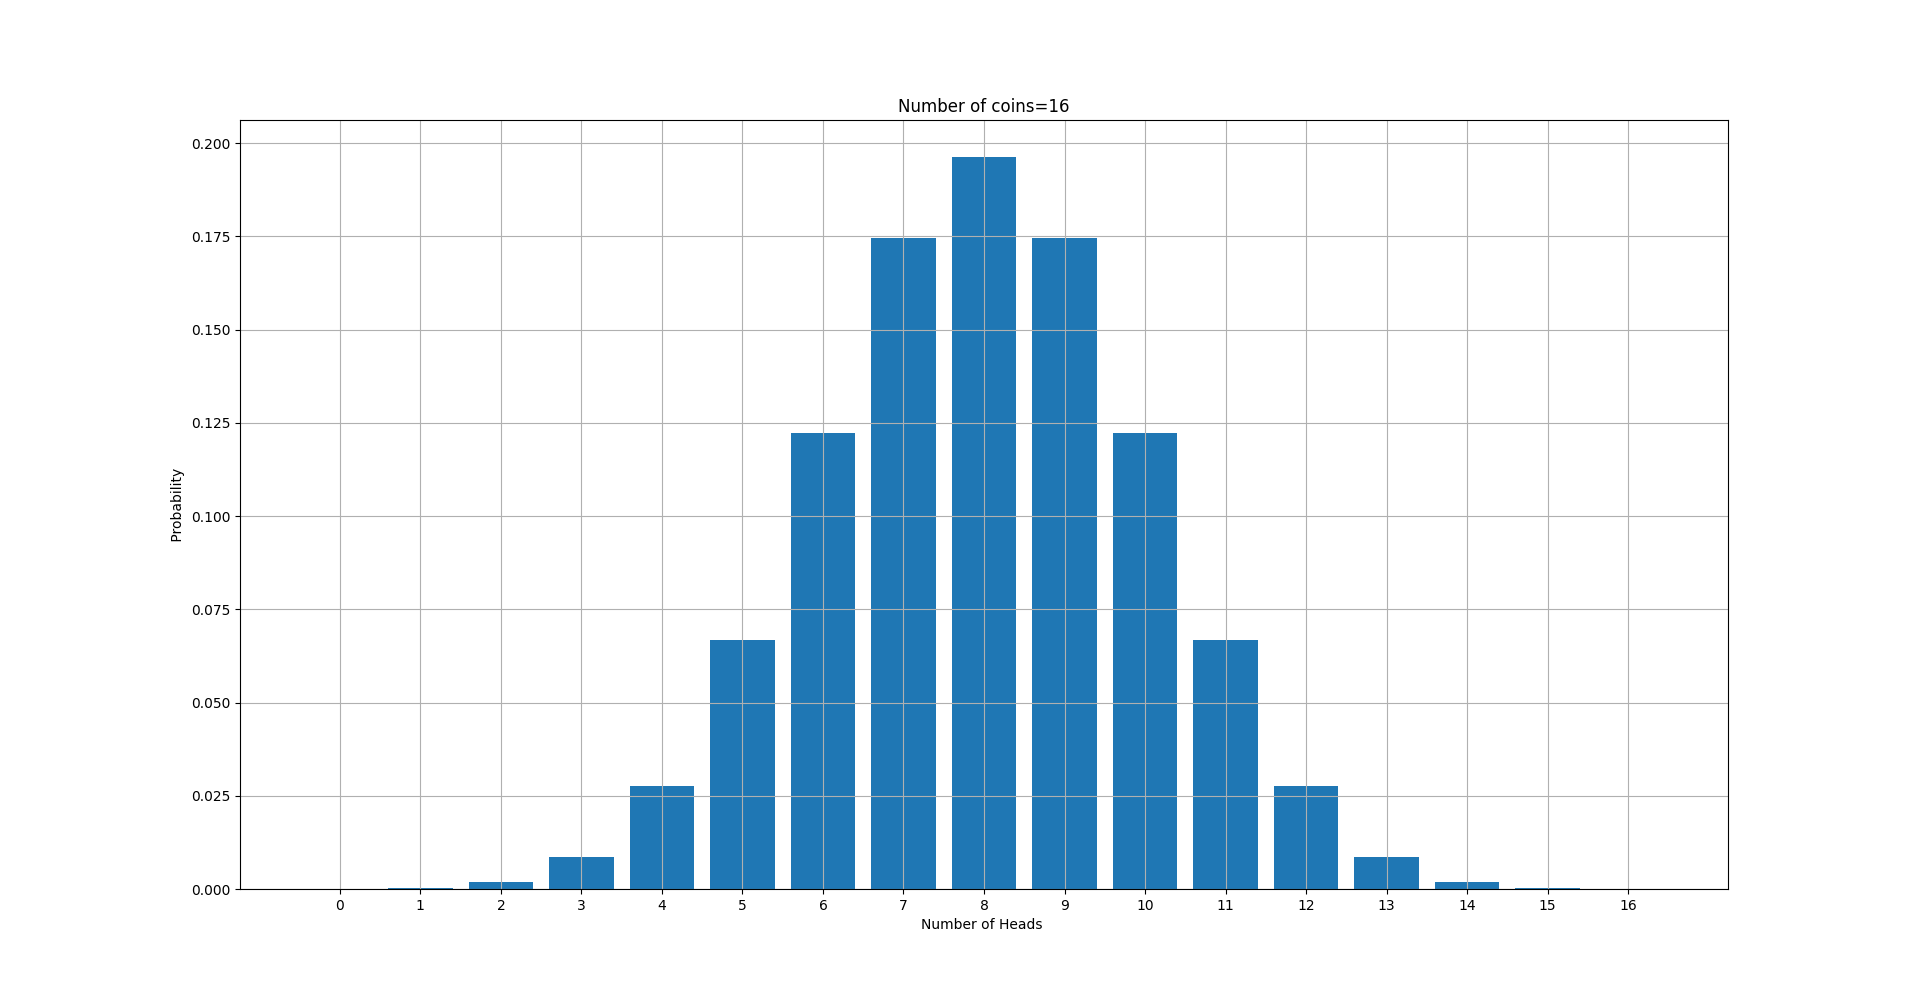
\includegraphics[width=15 cm]{prac_2_fig.png}
	
	%-------------------------------------------------------------------------------------
	
	\textbf{Program 2. Computation of the partition function Z(b) for the systems with a finite number of single
		particle levels (e.g., 2 level, 3 level etc.) and finite number of non-interacting particles
		N under Maxwell-Boltzmann/ Fermi-Dirac/Bose Einstein statistics:
		a) Study the behavior of Z(b), average energy, C v , and entropy and its dependence upon the
		temperature, total number of particles N and the spectrum of single particle energy
		states.
		b) Plot the probability of occupancy of all the states w.r.t. temperature.}
	\inputminted{python}{prac_3_MB.py}
	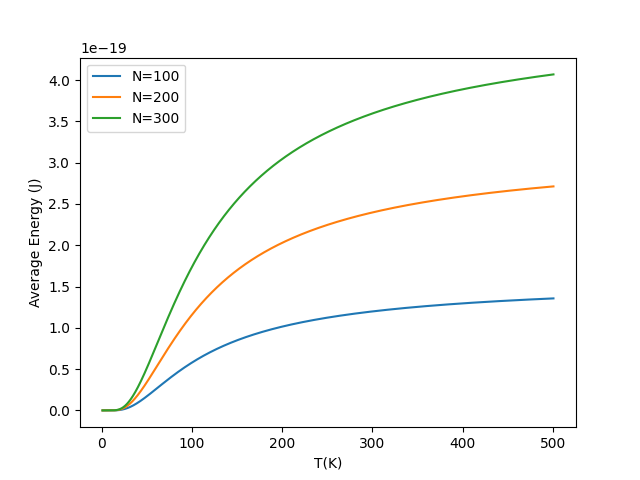
\includegraphics[width=15 cm]{MB_1.png}
	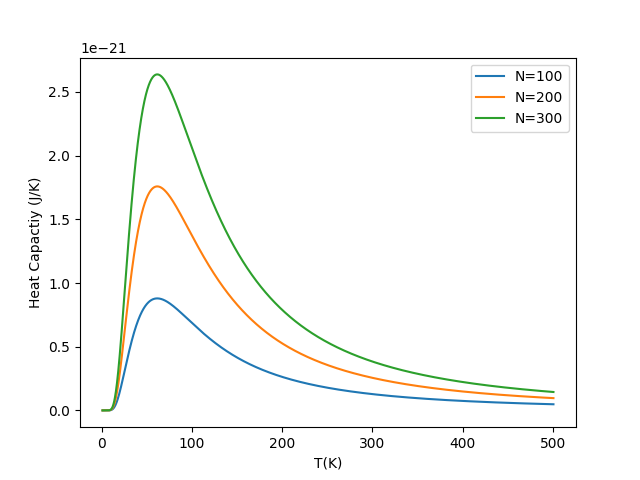
\includegraphics[width=15 cm]{MB_2.png}
	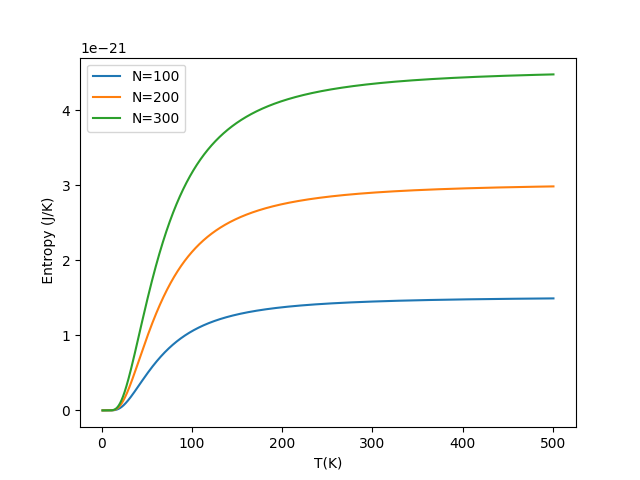
\includegraphics[width=15 cm]{MB_3.png}
	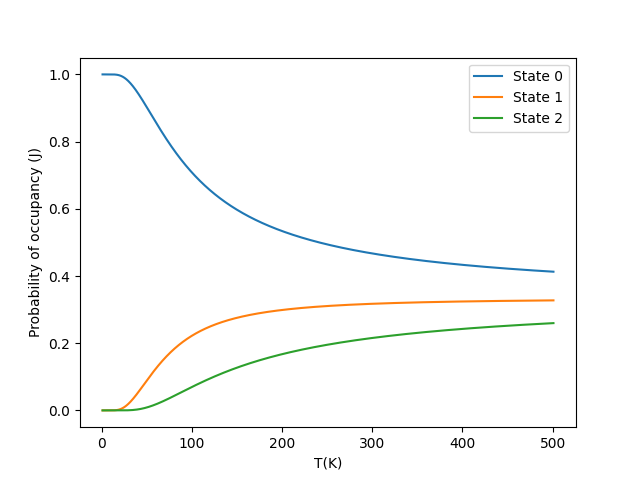
\includegraphics[width=15 cm]{MB_4.png}
	
	\inputminted{python}{prac_3_BE.py}
	
	\inputminted{python}{prac_3_FD.py}
	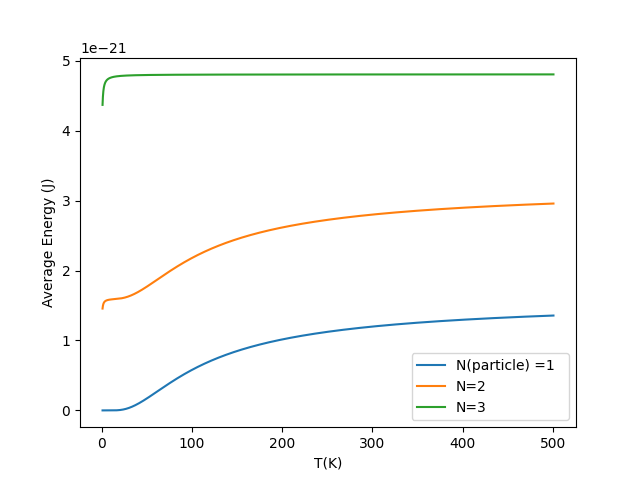
\includegraphics[width=15 cm]{FD_1.png}
	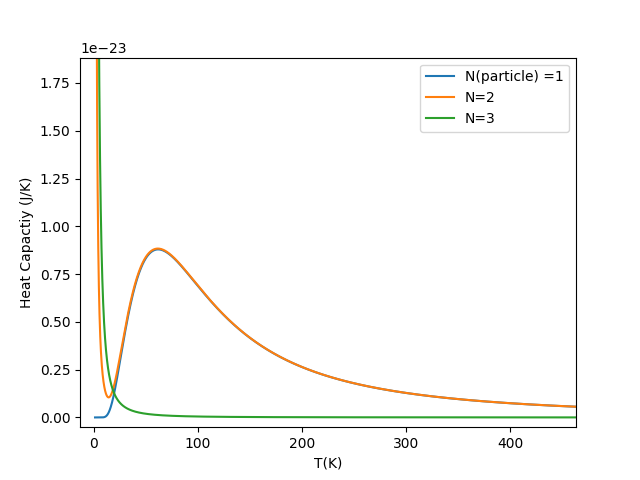
\includegraphics[width=15 cm]{FD_2.png}
	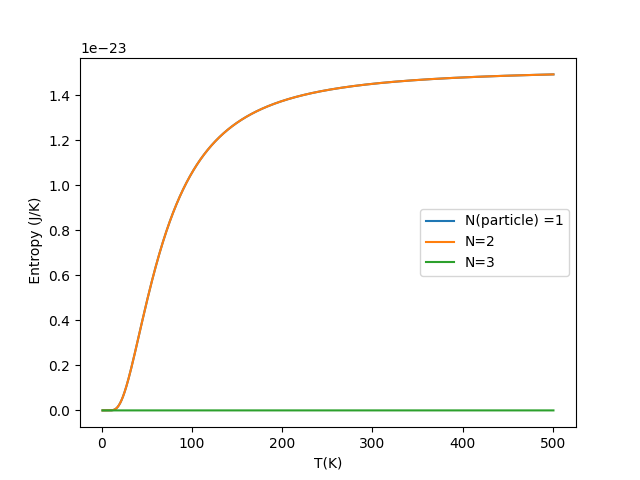
\includegraphics[width=15 cm]{FD_3.png}
	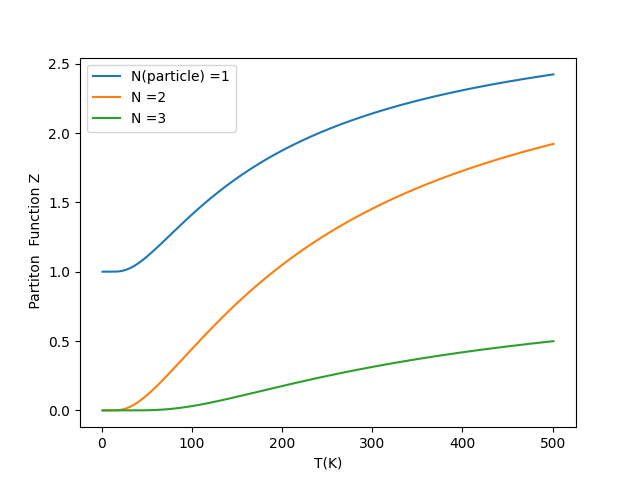
\includegraphics[width=15 cm]{FD_5.png}
	%-------------------------------------------------------------------------------------

	\textbf{Program 3. Plot the Maxwell speed distribution function at different temperatures in a 3-dimension
		system. Calculate the average speed, root mean square and most probable speed.}\\
	\inputminted{python}{prac_4.py}
	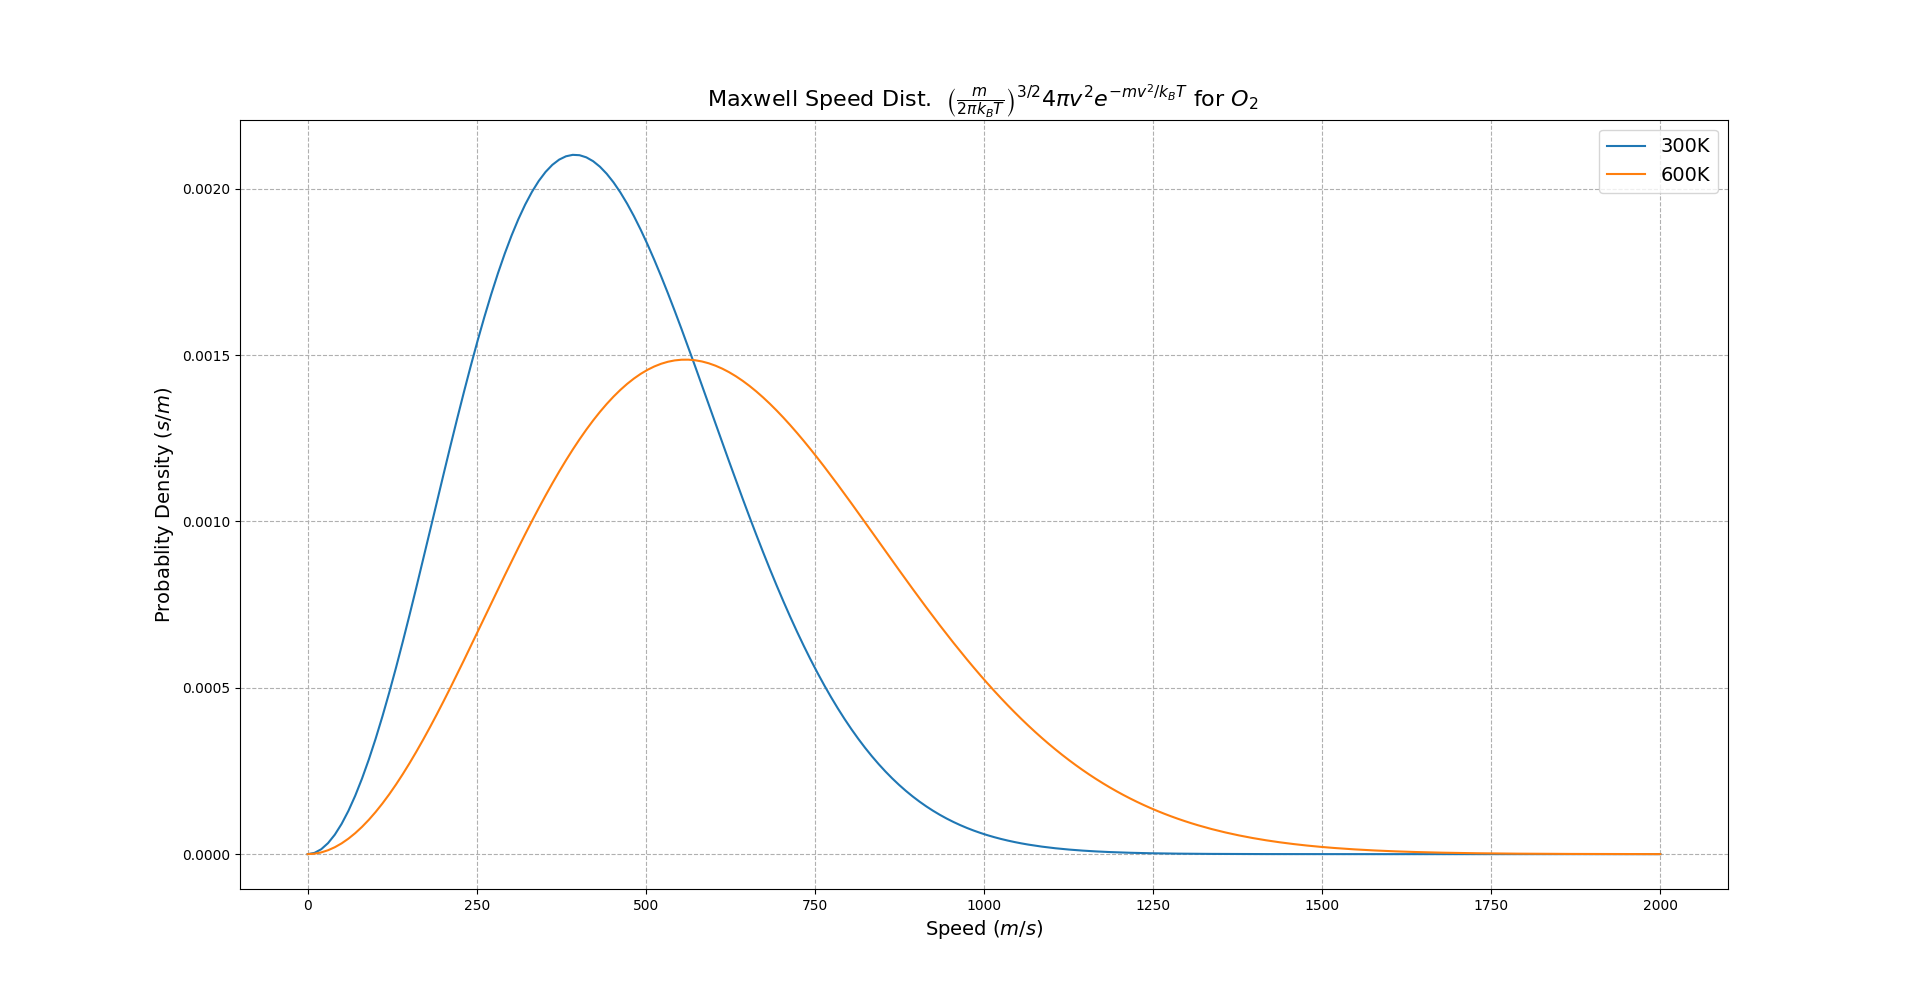
\includegraphics[width=15 cm]{prac_4_oxygen.png}
	%-------------------------------------------------------------------------------------

	\textbf{Program 4. Plot Specific Heat of Solids w.r.t temperature
		a) Dulong-Petit law,
		b) Einstein distribution function
		c) Debye distribution function}\\
	\inputminted{python}{prac_5.py}
	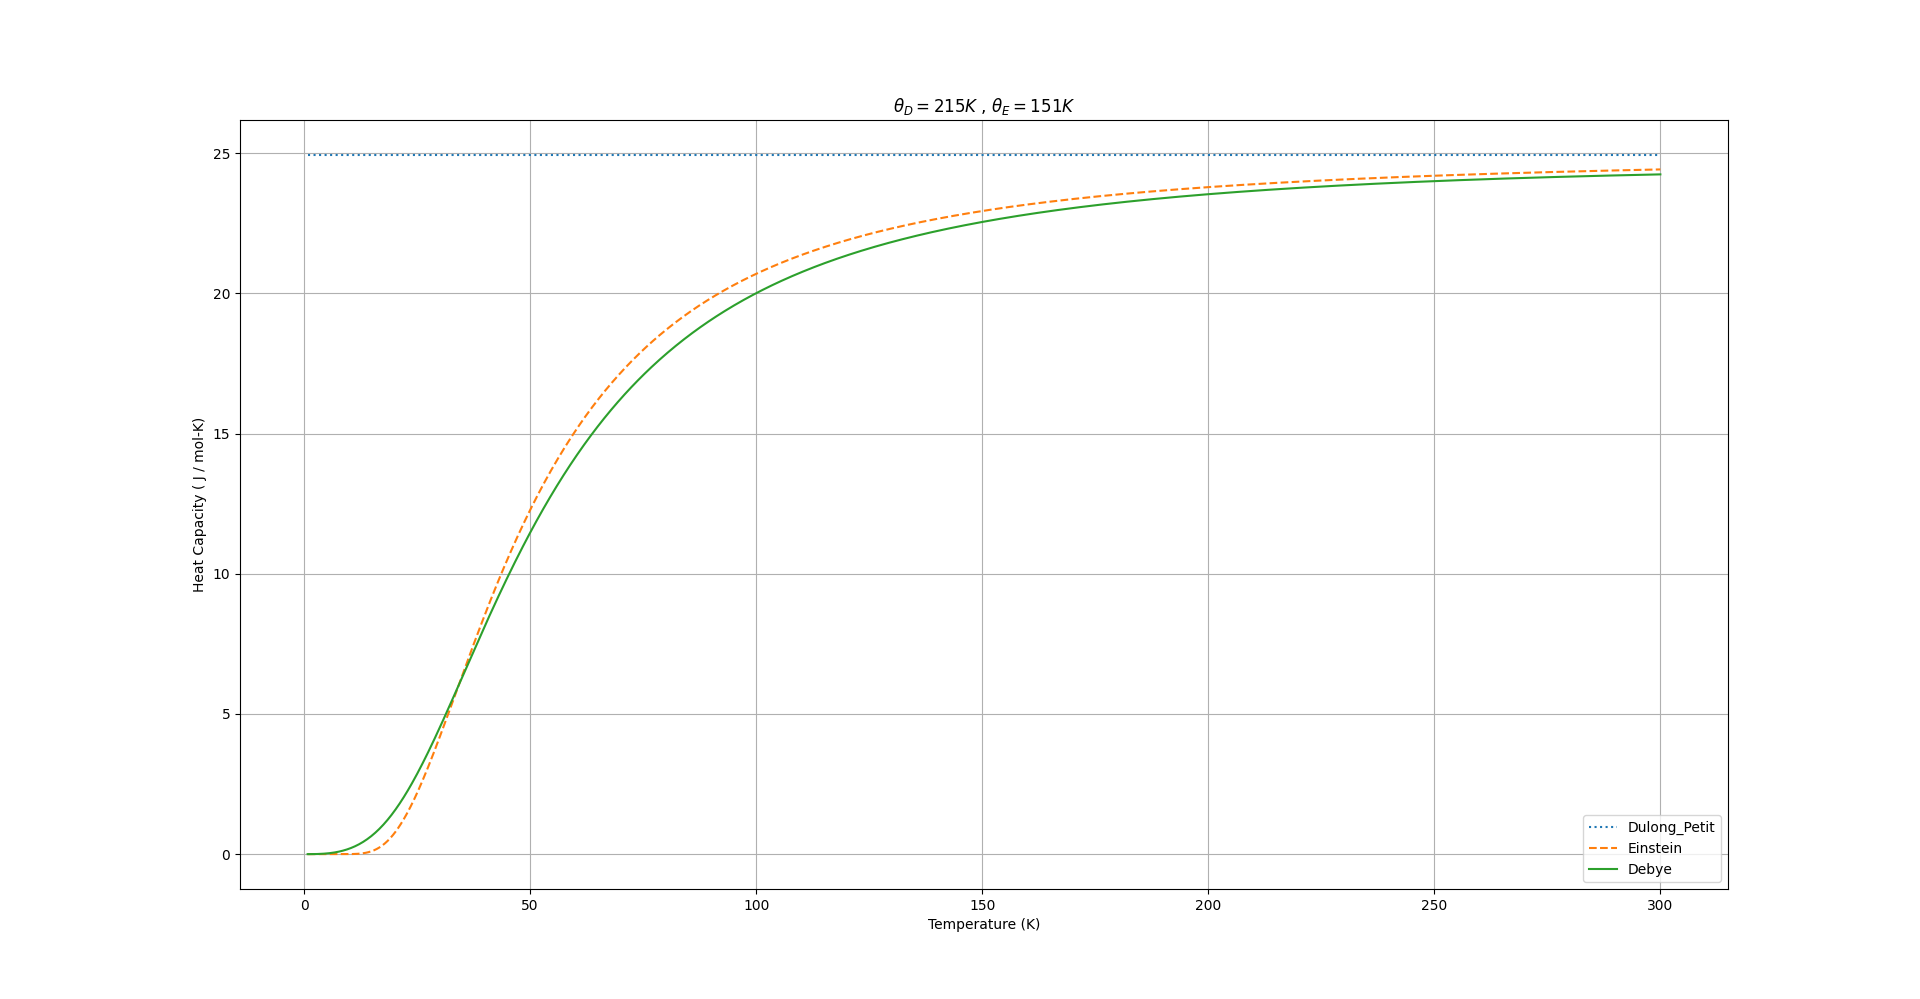
\includegraphics[width=15 cm]{prac_5.png}
	
	%-------------------------------------------------------------------------------------

	\textbf{Program 5. Plot the following functions with energy at different temperatures
		a) Maxwell-Boltzmann distribution
		b) Fermi-Dirac distribution
		c) Bose-Einstein distribution}\\
	\inputminted{python}{prac_6.py}
	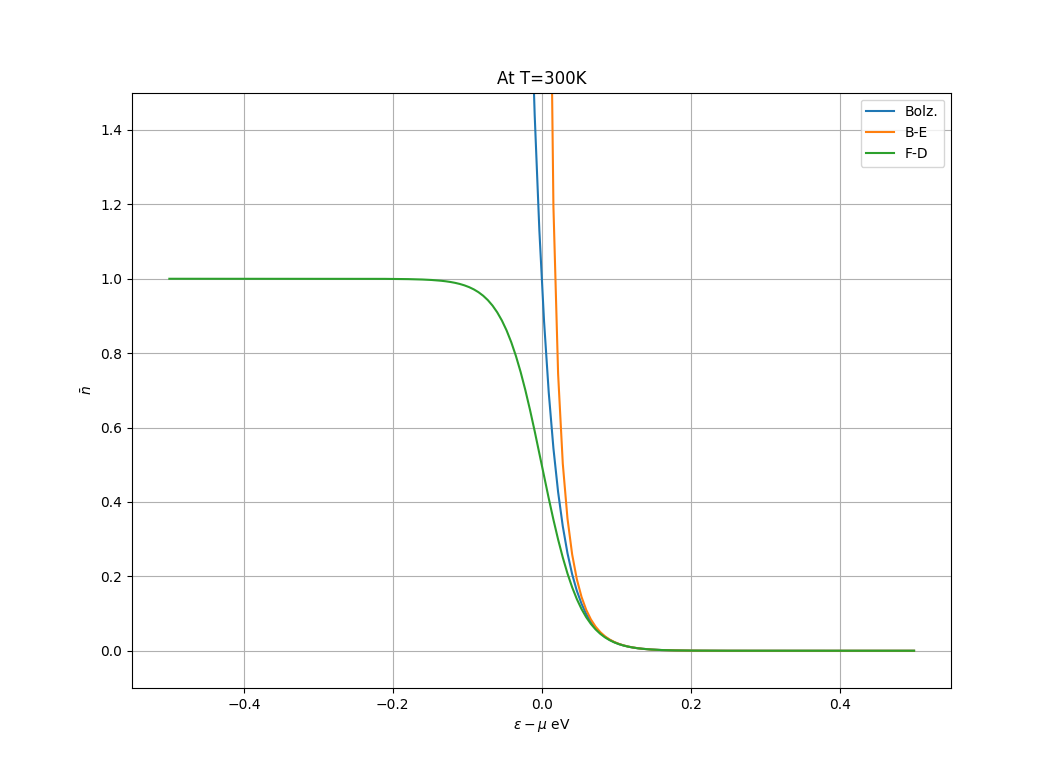
\includegraphics[width=15 cm]{prac_6_300k.png}
	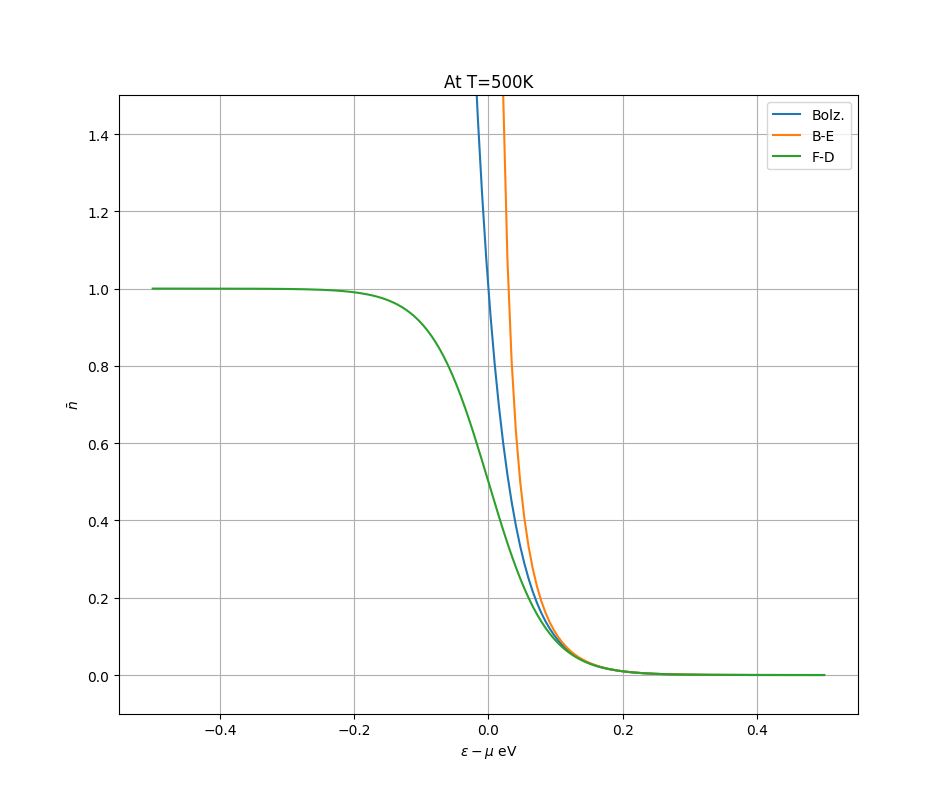
\includegraphics[width=15 cm]{prac_6_500k.png}
	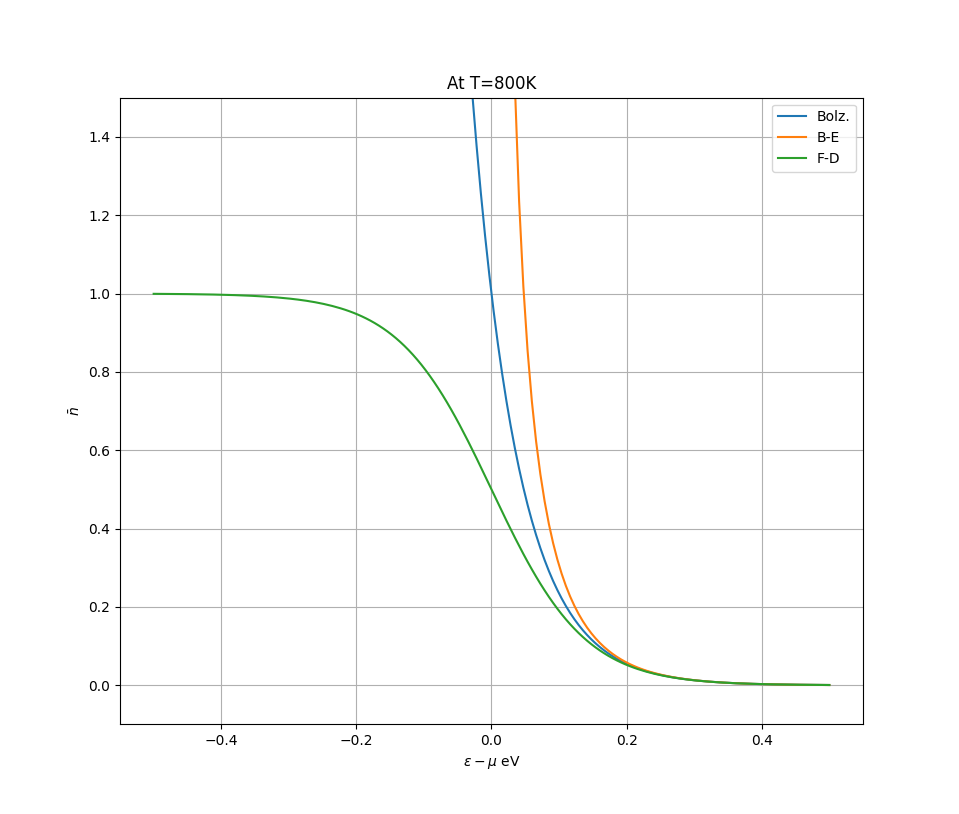
\includegraphics[width=15 cm]{prac_6_800k.png}
	%-------------------------------------------------------------------------------------

	\textbf{Program 6. Plot Planck’s law of Black body radiation w.r.t. wavelength/frequency at different
		temperatures. Compare it with Rayleigh-Jeans Law and Wien’s distribution law for a
		given temperature..}\\
	\inputminted{python}{prac_8.py}
	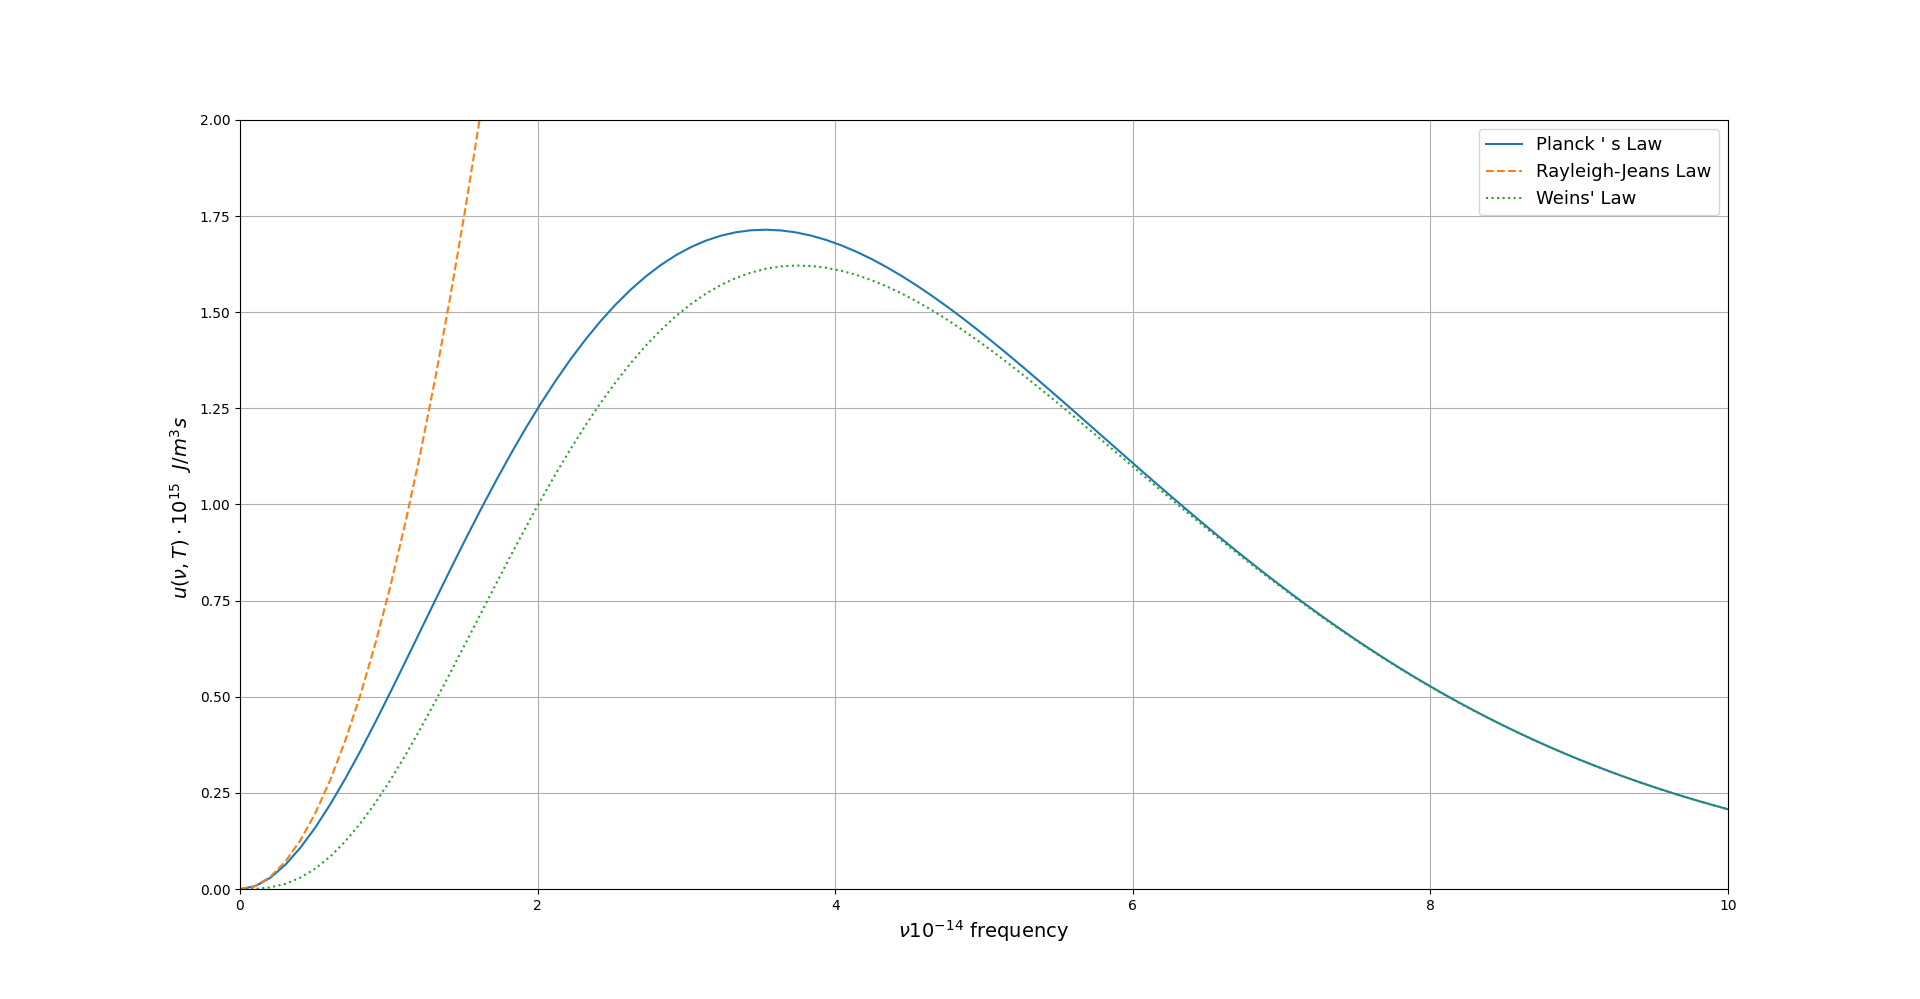
\includegraphics[width=15 cm]{prac_8.png}	
	%-------------------------------------------------------------------------------------
	
\end{document}